% chapters/08_teamwork.tex
\chapter{分工和协作}

\section*{本章团队协作速览}

\begin{table}[H]
    \centering
    \begin{tabular}{p{0.10\textwidth}p{0.20\textwidth}p{0.35\textwidth}p{0.25\textwidth}}
        \toprule
        \textbf{成员} & \textbf{角色定位} & \textbf{核心贡献领域} & \textbf{关键产出} \\
        \midrule
        潘利源 & 核心架构师 & 加密/完整性实现、内核集成、性能优化 & 7个补丁、约5000行Rust代码 \\
        陈韵 & 测试与文档工程师 & 性能测试框架、数据验证、技术文档撰写 & 测试脚本、技术文档 \\
        张乐桁 & 文档与运维工程师 & README文档、测试合同、基准脚本、PPT & README、答辩PPT、设计赛道文档 \\
        \bottomrule
    \end{tabular}
\end{table}

\section{队员信息}

\begin{table}[H]
    \centering
    \begin{tabular}{p{0.15\textwidth}p{0.25\textwidth}p{0.15\textwidth}p{0.35\textwidth}}
        \toprule
        \textbf{姓名} & \textbf{学校} & \textbf{队伍角色} & \textbf{主要职责} \\
        \midrule
        潘利源 & 华南师范大学 & 核心开发 & 核心加解密/完整性实现、星绽内核集成、性能优化、补丁制作 \\
        陈韵（jqtxzs） & 华南师范大学 & 测试与文档 & 性能测试框架增强、测试数据收集与验证、技术文档撰写 \\
        张乐桁（lehengzhang） & 华南师范大学 & 文档与运维 & README文档、性能测试合同编写、FIO/Filebench/SQLite/Boot脚本及证据目录整理、答辩PPT \\
        \bottomrule
    \end{tabular}
\end{table}

\section{分工详情}

\subsection{潘利源（核心架构师）}

\textbf{核心加密与完整性实现}（约2000行Rust）：
\begin{itemize}
    \item 实现 \texttt{BlockDevice} trait 及 \texttt{MemoryBlockDevice}、\texttt{FileBlockDevice} 后端；
    \item 实现纯 Rust SHA-256（\texttt{sha256.rs}，约120行）和 Merkle 哈希树（\texttt{hash\_tree.rs}，约150行）；
    \item 实现 AES-256-XTS 加密引擎及 Linux \texttt{aes-xts-plain64} 兼容性（\texttt{crypto.rs}、\texttt{dm\_crypt.rs}，约350行）；
    \item 实现 \texttt{dm-verity} 完整校验逻辑（\texttt{dm\_verity.rs}，约200行）；
    \item 实现 \texttt{DmStackBuilder} 可组合映射器链（\texttt{device\_mapper.rs}，约180行）。
\end{itemize}

\textbf{星绽内核集成}（约2500行Rust内核代码）：
\begin{itemize}
    \item 制作并维护 \texttt{\seqsplit{asterinas\_port/patches/0001--0007}} 全部7个补丁；
    \item 实现 BIO 路径适配（\texttt{device.rs}）、启动参数解析（\texttt{lib.rs}）、根文件系统切换（\texttt{pivot\_root}）；
    \item 实现 \texttt{/dev/mapper/control} 控制节点（\texttt{dm\_control.rs}，约520行）和运行时mapper管理（\texttt{runtime.rs}，约260行）；
    \item 实现组合栈（\texttt{dm\_stack=crypt,verity}，补丁0007）。
\end{itemize}

\textbf{性能优化}（约800行Rust）：
\begin{itemize}
    \item 实现 AES-NI 硬件加速（\texttt{\seqsplit{ostd/aesni.rs}}，约174行）及 FPU/XMM 状态保护；
    \item 实现有界临时缓冲池（scratch pool）减少动态分配；
    \item 实现认证后哈希缓存和 BIO 数据复用（\texttt{verity.rs}）；
    \item 实现内核性能统计接口（\texttt{/proc/dm-performance-stats}、\texttt{/proc/dm-verity-stats}）。
\end{itemize}

\textbf{核心产出}：约5000行Rust代码、7个内核补丁、17+个Git commits。

\textbf{代表性提交}：\texttt{40a52179}（初始dm实现）、\texttt{6385e70b}（组合栈）、\texttt{e07ad006}（KVM基准证据）。

\subsection{陈韵（jqtxzs，测试与文档工程师）}

\textbf{性能测试框架增强}（约400行Rust/Shell）：
\begin{itemize}
    \item 增强 \texttt{dmctl} 性能测试框架，支持 I/O 拆分解与可配置规模（commit \texttt{40d8abba}）；
    \item 更新性能测试数据与优化量化说明（commit \texttt{21aa566d}）；
    \item 统一正式性能口径并补充优化证据（协助）。
\end{itemize}

\textbf{测试数据与文档完善}：
\begin{itemize}
    \item 完善安全存储性能验证与交付材料（协助 commit \texttt{ca5afe46}）；
    \item 撰写并修改完善技术文档（commits \texttt{7350e470}、\texttt{dde97a2f}、\texttt{a975b887}、\texttt{bf9861b9}、\texttt{5dc3cb9f}、\texttt{29157f0e}）；
    \item 完善更新图表（commit \texttt{8b2018e7}）。
\end{itemize}

\textbf{核心产出}：6+个Git commits、性能测试框架增强、技术文档（与潘利源协作完成技术内容审阅）。

\textbf{代表性提交}：\texttt{40d8abba}（性能框架增强）、\texttt{7350e470}（技术文档撰写）。

\subsection{张乐桁（lehengzhang，文档与运维工程师）}

\textbf{性能测试合同与基准脚本}（约1000行Shell/Python）：
\begin{itemize}
    \item 编写 \texttt{\seqsplit{docs/benchmark\_contract.md}} 定义正式性能测试合同（包含环境、FIO参数、元数据等完整规范）；
    \item 整理 FIO、Filebench、SQLite、Boot 测试脚本及证据目录（commit \texttt{1ac6325c}）；
    \item 维护 \texttt{\seqsplit{scripts/run\_fio\_matrix.sh}}、\texttt{\seqsplit{scripts/run\_filebench\_matrix.sh}}、\texttt{\seqsplit{scripts/run\_sqlite\_matrix.sh}}、\texttt{\seqsplit{scripts/run\_boot\_matrix.sh}} 等核心基准脚本。
\end{itemize}

\textbf{README与答辩材料}（LaTeX/Markdown + PPT）：
\begin{itemize}
    \item 撰写并维护项目根目录 \texttt{README.md}，包含快速验证指南、功能命令、性能结果和验收说明；
    \item 添加 LaTeX 文档框架与答辩 PPT（commit \texttt{f5878935}）；
    \item 将答辩 PPT 放到项目根目录并更新 README 链接（commit \texttt{dabfee4d}）；
    \item 在 README 开头添加演示视频百度网盘链接（commit \texttt{c22b8b47}）；
    \item 完成最终文档整合与数据对齐（包括技术文档重编、设计文档整合等），并于 08-18 完成全部答辩材料提交。
\end{itemize}

\textbf{核心产出}：多个Git commits、README文档、设计赛道文档、答辩PPT。

\textbf{代表性提交}：\texttt{f5878935}（LaTeX文档框架与PPT）、\texttt{1ac6325c}（性能测试合同与脚本）、\texttt{1f4d9c11}（正式文档改为 design\_doc）。

\section{协作方式}

\subsection{版本管理}

\begin{itemize}
    \item 使用 \textbf{GitLab} 作为代码托管平台，所有代码提交均通过 Git 进行版本管理；
    \item 采用主分支开发模式，重要功能通过补丁序列（\texttt{\seqsplit{asterinas\_port/patches/}}）独立演进，便于审计和回溯；
    \item 提交信息遵循约定格式（\texttt{feat:}、\texttt{fix:}、\texttt{docs:} 前缀），关键提交包含功能描述和关联问题；
    \item 累计提交67次，覆盖从初始框架到最终交付的完整历程。
\end{itemize}

\textbf{关键迭代节点说明}：
\begin{enumerate}
    \item \textbf{基础架构与核心逻辑}（Commit \texttt{40a52179}）：完成了 \texttt{BlockDevice} trait 的抽象，实现了纯 Rust 的 AES-256-XTS 加密与 SHA-256 默克尔树校验。
    \item \textbf{内核集成与 BIO 路径打通}（Commit \texttt{c72462b2}、\texttt{2f8a6711}）：将用户态逻辑移植至星绽内核，成功实现了基于 \texttt{pivot\_root} 的受保护根文件系统切换。
    \item \textbf{性能对照与验收证据}（Commit \texttt{5f345a18}）：完成安全存储性能对照，包括正式 256 MiB 五轮基准、Linux guest 同条件对照、启动时间测量和哈希缓存 A/B 验证。
    \item \textbf{性能优化与基准固化}（Commits \texttt{e07ad006}、\texttt{c1f9c472}、\texttt{40d8abba}、\texttt{ca5afe46}、\texttt{5717d925}）：固化 KVM 基准证据，优化 dm 热路径，增强 \texttt{dmctl} 性能测试框架，更新完成队列性能指标与证据。
    \item \textbf{最终评测整合}（Commits \texttt{1ac6325c} 至 \texttt{8b2018e7}，08-09 至 08-11）：整理性能测试合同与 FIO/Filebench/SQLite/Boot 脚本及证据目录，统一正式性能口径，修正运行时能力声明并补充 KVM 回归验证，整合最终评测代码与测试材料并合并 GitLab 最新代码。
    \item \textbf{文档与合规性完善}（Commits \texttt{84970aae}、\texttt{f5878935}、\texttt{7350e470}、\texttt{dde97a2f}、\texttt{1f4d9c11} 等）：全面梳理技术文档，完成中文化翻译，补充 AI 工具使用声明，并添加 LaTeX 技术文档和答辩 PPT；8月16-18日完成最终文档整合（统一为 \texttt{design\_doc}）及答辩材料提交。
\end{enumerate}

\subsection{沟通与同步}

\begin{itemize}
    \item 每周通过线上会议（腾讯会议/钉钉）同步开发进度，每次会议约1小时，讨论架构决策、问题排查和下周计划；
    \item 使用即时通讯工具（QQ/微信）进行日常技术交流和问题排查，平均每天有3-5条技术消息交流；
    \item 重要技术决策（如 BIO 生命周期设计、缓存安全策略）在会议中集体讨论后实施，形成共识文档；
    \item 关键问题（如性能测试真实性问题、\texttt{pivot\_root}限制）通过紧急会议快速解决。
\end{itemize}

\subsection{代码审查}

\begin{itemize}
    \item 核心模块（加密、校验、BIO 处理）的代码变更须至少一名其他成员审查后方可合并；
    \item 补丁提交前，在本地进行完整的 \texttt{cargo test} 和 KVM 正确性验证；
    \item 性能相关的脚本和配置变更需通过 \texttt{\seqsplit{check\_benchmark\_package.py}} 静态检查；
    \item 文档变更（README、技术文档）在合并前进行交叉审阅，确保表述准确、无歧义。
\end{itemize}

\subsection{决策机制}

项目采用“共识驱动”的决策模式，关键决策均经过充分讨论：

\begin{itemize}
    \item \textbf{技术方案决策}：由提出者阐述方案（含优缺点分析），全体成员讨论后投票表决；
    \item \textbf{架构方向决策}：需形成书面决策记录（如补丁设计说明），确保决策可追溯；
    \item \textbf{紧急问题决策}：由核心开发者（潘利源）快速决策并实施修复，事后在周会上说明。
\end{itemize}

\subsection{关键决策记录}

\begin{table}[H]
    \centering
    \small
    \caption{关键技术决策记录}
    \begin{tabular}{p{0.15\textwidth}p{0.25\textwidth}p{0.25\textwidth}p{0.25\textwidth}}
        \toprule
        \textbf{时间} & \textbf{决策事项} & \textbf{决策结果} & \textbf{决策依据} \\
        \midrule
        06-23 & \texttt{BlockDevice} trait 设计 & 采用同步接口（内核用BIO封装） & 统一抽象、简化用户态测试 \\
        07-01 & AES-XTS实现方式 & 独立实现而非依赖RustCrypto xts-mode & 减少依赖、便于逐字节调优 \\
        07-10 & 补丁组织方式 & 7个独立补丁渐进式集成 & 可审计、可回退、每步可验证 \\
        07-15 & 性能优化优先级 & AES-NI > hash cache > scratch pool & 硬件加速收益最大、风险最低 \\
        08-05 & 数据真实性处理 & 废弃旧批次、重新执行 & 数据诚信优先于“好看” \\
        08-10 & 文档语言 & 中文（部分术语保留英文） & 便于评委阅读、关键术语准确 \\
        \bottomrule
    \end{tabular}
\end{table}

\section{AI 工具辅助协作}

项目开发过程中合理使用了 AI 辅助工具（详见 \texttt{\seqsplit{docs/ai\_tool\_disclosure.md}}），具体使用场景包括：

\begin{table}[H]
    \centering
    \caption{AI 工具使用详情}
    \begin{tabular}{p{0.15\textwidth}p{0.15\textwidth}p{0.60\textwidth}}
        \toprule
        \textbf{工具名称} & \textbf{相关大模型} & \textbf{具体使用场景与辅助内容} \\
        \midrule
        Cursor & Composer 2.5 & 1. 全盘检索答辩素材（PPT、PDF、图片、文本等）并核对清单；\\
         & & 2. 按答辩四段结构将14个素材文件分类归档至 \texttt{答辩PPT素材/} 目录；\\
         & & 3. 辅助整理答辩 PPT 的素材组织结构。\\
        \midrule
        Claude Code & GLM 5.2 & 1. 深度审查 dm-crypt 实现，重点检查 AES-256-XTS 的 tweak 计算、扇区号换算、加解密对称性与边界条件；\\
         & & 2. 与 Asterinas 内核侧实现及 Linux dm-crypt/cryptsetup 语义交叉比对，验证核心算法正确性；\\
         & & 3. 输出结构化审查报告，列出 \texttt{iv\_large\_sectors} 被静默接受、缺少已知答案测试（KAT）等6项潜在问题及验证方法；\\
         & & 4. 给出修复优先级建议，并提供相应补丁与 NIST KAT 测试用例供人工审阅取舍。\\
        \midrule
        通义千问（Qwen） & Qwen-Max & 技术文档的深度润色，确保中英文专业术语的准确性与一致性。 \\
        \midrule
        豆包（Doubao） & 豆包大模型 & 答辩表述的逻辑优化，整理技术答辩常见问题及应对策略。 \\
        \midrule
        WorkBuddy & 腾讯混元 Hy3、DeepSeek & 辅助执行测试、完整内核构建和 QEMU 验证并解读日志。 \\
        \bottomrule
    \end{tabular}
\end{table}

\textbf{AI 交互记录}：以下是开发过程中与 AI 工具的关键交互截图，证明 AI 仅作为辅助工具，开发逻辑由团队主导。

\subsubsection{Cursor（Composer 2.5）交互记录}

\begin{figure}[H]
    \centering
    \includegraphics[width=0.9\textwidth]{cursor_ai_1.png}
    \caption{Cursor（Composer 2.5）检索答辩素材并按四段结构分类归档}
    \label{fig:cursor_1}
\end{figure}

\subsubsection{Claude Code（GLM 5.2）交互记录}

\begin{figure}[H]
    \centering
    \includegraphics[width=0.95\textwidth]{claude_code_ai_1.png}
    \caption{Claude Code（GLM 5.2）dm-crypt 审查：核心算法验证符合 IEEE 1619 / plain64 语义}
    \label{fig:claude_code_1}
\end{figure}

\begin{figure}[H]
    \centering
    \includegraphics[width=0.95\textwidth]{claude_code_ai_2.png}
    \caption{Claude Code（GLM 5.2）潜在问题列表与验证方法}
    \label{fig:claude_code_2}
\end{figure}

\begin{figure}[H]
    \centering
    \includegraphics[width=0.95\textwidth]{claude_code_ai_3.png}
    \caption{Claude Code（GLM 5.2）修复优先级建议}
    \label{fig:claude_code_3}
\end{figure}

\subsubsection{通义千问（Qwen）交互记录}

\begin{figure}[H]
    \centering
    \begin{subfigure}[b]{0.45\textwidth}
        \centering
        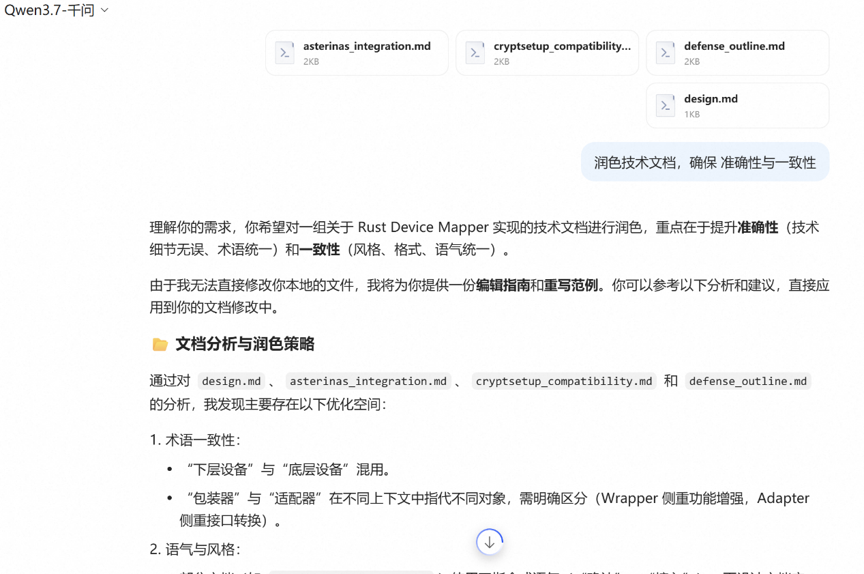
\includegraphics[width=\textwidth]{qwen_ai_1.png}
        \caption{技术文档润色}
        \label{fig:qwen_1}
    \end{subfigure}
    \hfill
    \begin{subfigure}[b]{0.45\textwidth}
        \centering
        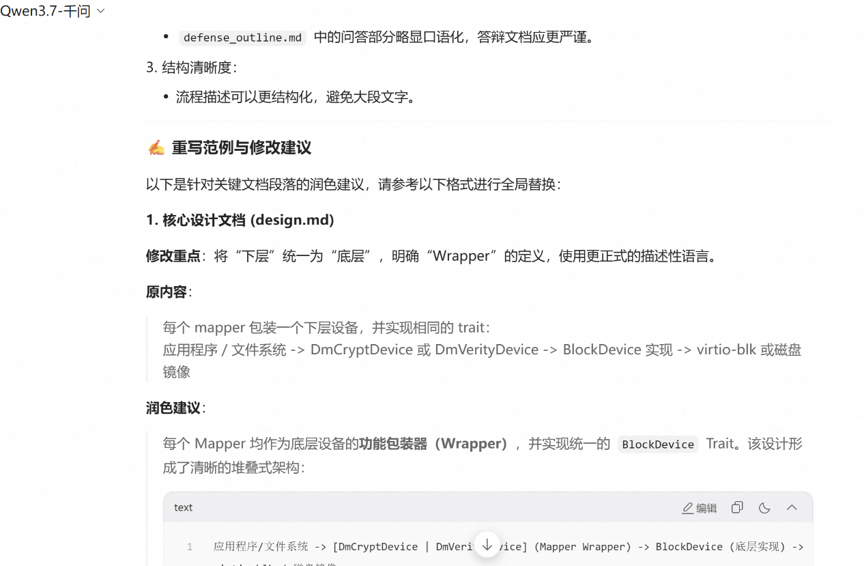
\includegraphics[width=\textwidth]{qwen_ai_2.png}
        \caption{专业术语校对}
        \label{fig:qwen_2}
    \end{subfigure}
    \caption{通义千问（Qwen）交互记录}
    \label{fig:qwen_group}
\end{figure}

\subsubsection{豆包（Doubao）交互记录}

\begin{figure}[H]
    \centering
    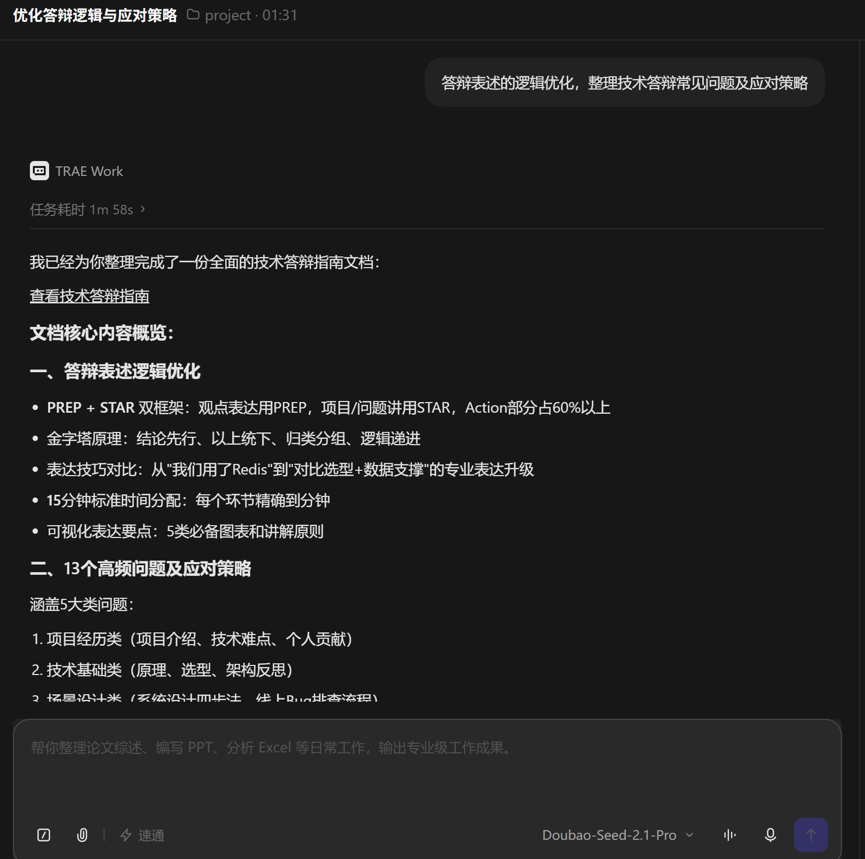
\includegraphics[width=0.8\textwidth]{doubao_ai_1.png}
    \caption{豆包（Doubao）答辩表述优化与 FAQ 整理}
    \label{fig:doubao_1}
\end{figure}

\textbf{验证机制与责任声明}：
\begin{enumerate}
    \item \textbf{人工审查}：所有 AI 生成的代码片段和文档内容，均经过团队成员的人工 Peer Review。
    \item \textbf{交叉验证}：代码正确性通过严格的单元测试、与 Linux dm-crypt 的逐字节对照、星绽内核构建及 QEMU 端到端运行进行了多重验证。
    \item \textbf{责任承担}：最终的技术方案、代码取舍、架构决策和提交材料均由参赛团队全权负责。
\end{enumerate}

\section{Git 提交记录概览}

完整提交共 67 次，下表列出主要代表性提交（与 GitLab 仓库历史逐条对应），完整反映了项目的开发节奏和功能演进：

\begin{longtable}{p{0.05\textwidth}p{0.09\textwidth}p{0.13\textwidth}p{0.51\textwidth}p{0.12\textwidth}}
    \caption{Git 提交记录概览} \\
    \toprule
    \textbf{序号} & \textbf{日期} & \textbf{Commit Hash} & \textbf{提交说明} & \textbf{作者} \\
    \midrule
    \endfirsthead
    \caption[]{Git 提交记录概览（续）} \\
    \toprule
    \textbf{序号} & \textbf{日期} & \textbf{Commit Hash} & \textbf{提交说明} & \textbf{作者} \\
    \midrule
    \endhead
    \midrule
    \multicolumn{5}{r}{\small 接下一页} \\
    \endfoot
    \bottomrule
    \endlastfoot
    1 & 06-23 & \texttt{6bb9bc92} & 初始提交，仅源码，屏蔽编译产物 & 潘利源 \\
    2 & 06-23 & \texttt{40a52179} & feat: add Linux-compatible device mapper implementation & 潘利源 \\
    3 & 06-23 & \texttt{c72462b2} & fix: validate Asterinas dm BIO paths & 潘利源 \\
    4 & 06-23 & \texttt{2f8a6711} & 接入受保护根文件系统并完善项目文档 & 潘利源 \\
    5 & 06-23 & \texttt{a0dbb0f5} & 补充国产 AI 工具使用说明 & 潘利源 \\
    6 & 06-23 & \texttt{84970aae} & 修改文档 & 潘利源 \\
    7 & 06-29 & \texttt{f5878935} & 添加 LaTeX 项目文档、PDF 与答辩 PPT & 张乐桁 \\
    8 & 06-29 & \texttt{dabfee4d} & 将答辩 PPT 放到项目根目录并更新 README 链接 & 张乐桁 \\
    9 & 06-29 & \texttt{c22b8b47} & 在 README 开头添加演示视频百度网盘链接 & 张乐桁 \\
    10 & 07-14 & \texttt{5f345a18} & 完成安全存储性能对照与国赛验收证据 & 潘利源 \\
    11 & 07-25 & \texttt{e07ad006} & 修正评审材料并固化 KVM 基准证据 & 潘利源 \\
    12 & 07-28 & \texttt{c1f9c472} & 优化 dm 热路径并补齐评审基准流程 & 潘利源 \\
    13 & 08-03 & \texttt{40d8abba} & 增强 dmctl 性能测试框架，支持 IO 拆分解与可配置规模 & 陈韵 \\
    14 & 08-03 & \texttt{ca5afe46} & 完善安全存储性能验证与交付材料 & 潘利源 \\
    15 & 08-06 & \texttt{5717d925} & 更新 dm 完成队列性能指标与证据 & 潘利源 \\
    16 & 08-09 & \texttt{21aa566d} & 更新性能测试数据与优化量化说明 & 陈韵 \\
    17 & 08-09 & \texttt{6926b356} & change & 陈韵 \\
    18 & 08-09 & \texttt{7431e5de} & 统一正式性能口径并补充优化证据 & 潘利源 \\
    19 & 08-09 & \texttt{0e7f4c77} & 修正运行时能力声明并补充 KVM 回归验证 & 潘利源 \\
    20 & 08-09 & \texttt{09f62e59} & 补充完整测试进度 & 潘利源 \\
    21 & 08-09 & \texttt{1ac6325c} & 整理性能测试合同、FIO/Filebench/SQLite/Boot 脚本与证据目录 & 张乐桁 \\
    22 & 08-10 & \texttt{fc548a9e} & 整合最终评测代码与测试材料 & 潘利源 \\
    23 & 08-10 & \texttt{7350e470} & 修改完善文档 & 陈韵 \\
    24 & 08-10 & \texttt{dde97a2f} & 更新完善技术文档内容 & 陈韵 \\
    25 & 08-11 & \texttt{6385e70b} & feat: add kernel Combined crypt→verity stack path & 潘利源 \\
    26 & 08-11 & \texttt{fda85aa4} & 整合最终评测代码与测试材料 & 潘利源 \\
    27 & 08-11 & \texttt{84fe076e} & 合并 GitLab 最新代码并同步最终评测材料 & 潘利源 \\
    28 & 08-11 & \texttt{8b2018e7} & 完善更新图表 & 陈韵 \\
    29 & 08-11 & \texttt{5dc3cb9f} & 上传设计文档内容 & 陈韵 \\
    30 & 08-11 & \texttt{29157f0e} & 整合更新commit记录 & 陈韵 \\
    31 & 08-12 & \texttt{a975b887} & 更新完善技术文档内容 & 陈韵 \\
    32 & 08-16 & \texttt{1f4d9c11} & docs: 正式文档改为 design\_doc，移除旧 main.tex/PDF & 张乐桁 \\
    33 & 08-16 & \texttt{c64c8ce7} & docs: 在报告中补入 Asterinas 256 MiB 三行表并重编 PDF & 张乐桁 \\
    34 & 08-16 & \texttt{d9b960f4} & docs: 用 Linux QEMU virtio FIO 替换宿主机对照数字 & 张乐桁 \\
    35 & 08-17 & \texttt{7cd6d8f1} & docs: 重编 document/main.pdf，测试指标与 README 对齐 & 张乐桁 \\
    36 & 08-17 & \texttt{97fcb8db} & docs: 按核对后的 Asterinas KVM FIO 13 格式更新 PDF & 张乐桁 \\
    37 & 08-17 & \texttt{d697645b} & docs: Asterinas KVM FIO 13 格式补入 raw 列 & 张乐桁 \\
    38 & 08-17 & \texttt{17f11f70} & docs: 写明 asterinas/软链接 Asterinas 官方仓库 & 张乐桁 \\
    39 & 08-17 & \texttt{bf9861b9} & 汇总成完整一个技术文档 & 陈韵 \\
    40 & 08-17 & \texttt{c8b5c9cf} & docs: 在 Linux guest 同条件对照表中补入 dm-verify & 张乐桁 \\
    41 & 08-17 & \texttt{da5fbae4} & docs: 恢复 main.pdf 并公布 Linux guest Filebench/SQLite 与 README 完成情况表 & 张乐桁 \\
    42 & 08-18 & \texttt{d56affa8} & docs: README 补全用户态与内核态说明 & 张乐桁 \\
    43 & 08-18 & \texttt{6e06b136} & docs: 补入 256 MiB 正式合同与 Linux guest 对照表 & 张乐桁 \\
    44 & 08-18 & \texttt{9894d4bf} & docs: 设计文档整合 & 张乐桁 \\
    45 & 08-18 & \texttt{a0b7aacf} & docs: FIO 表格修订为 qd=1 配置 & 张乐桁 \\
    46 & 08-18 & \texttt{72f6738c} & docs: FIO 表格进一步修订 & 张乐桁 \\
    47 & 08-18 & \texttt{ef345837} & docs: 最终 README 更新 & 张乐桁 \\
    48 & 08-18 & \texttt{b3247e0e} & test: 全量测试通过 & 潘利源 \\
\end{longtable}

\textbf{Git 提交历史截图}：

\begin{figure}[H]
    \centering
    \begin{subfigure}[b]{0.48\textwidth}
        \centering
        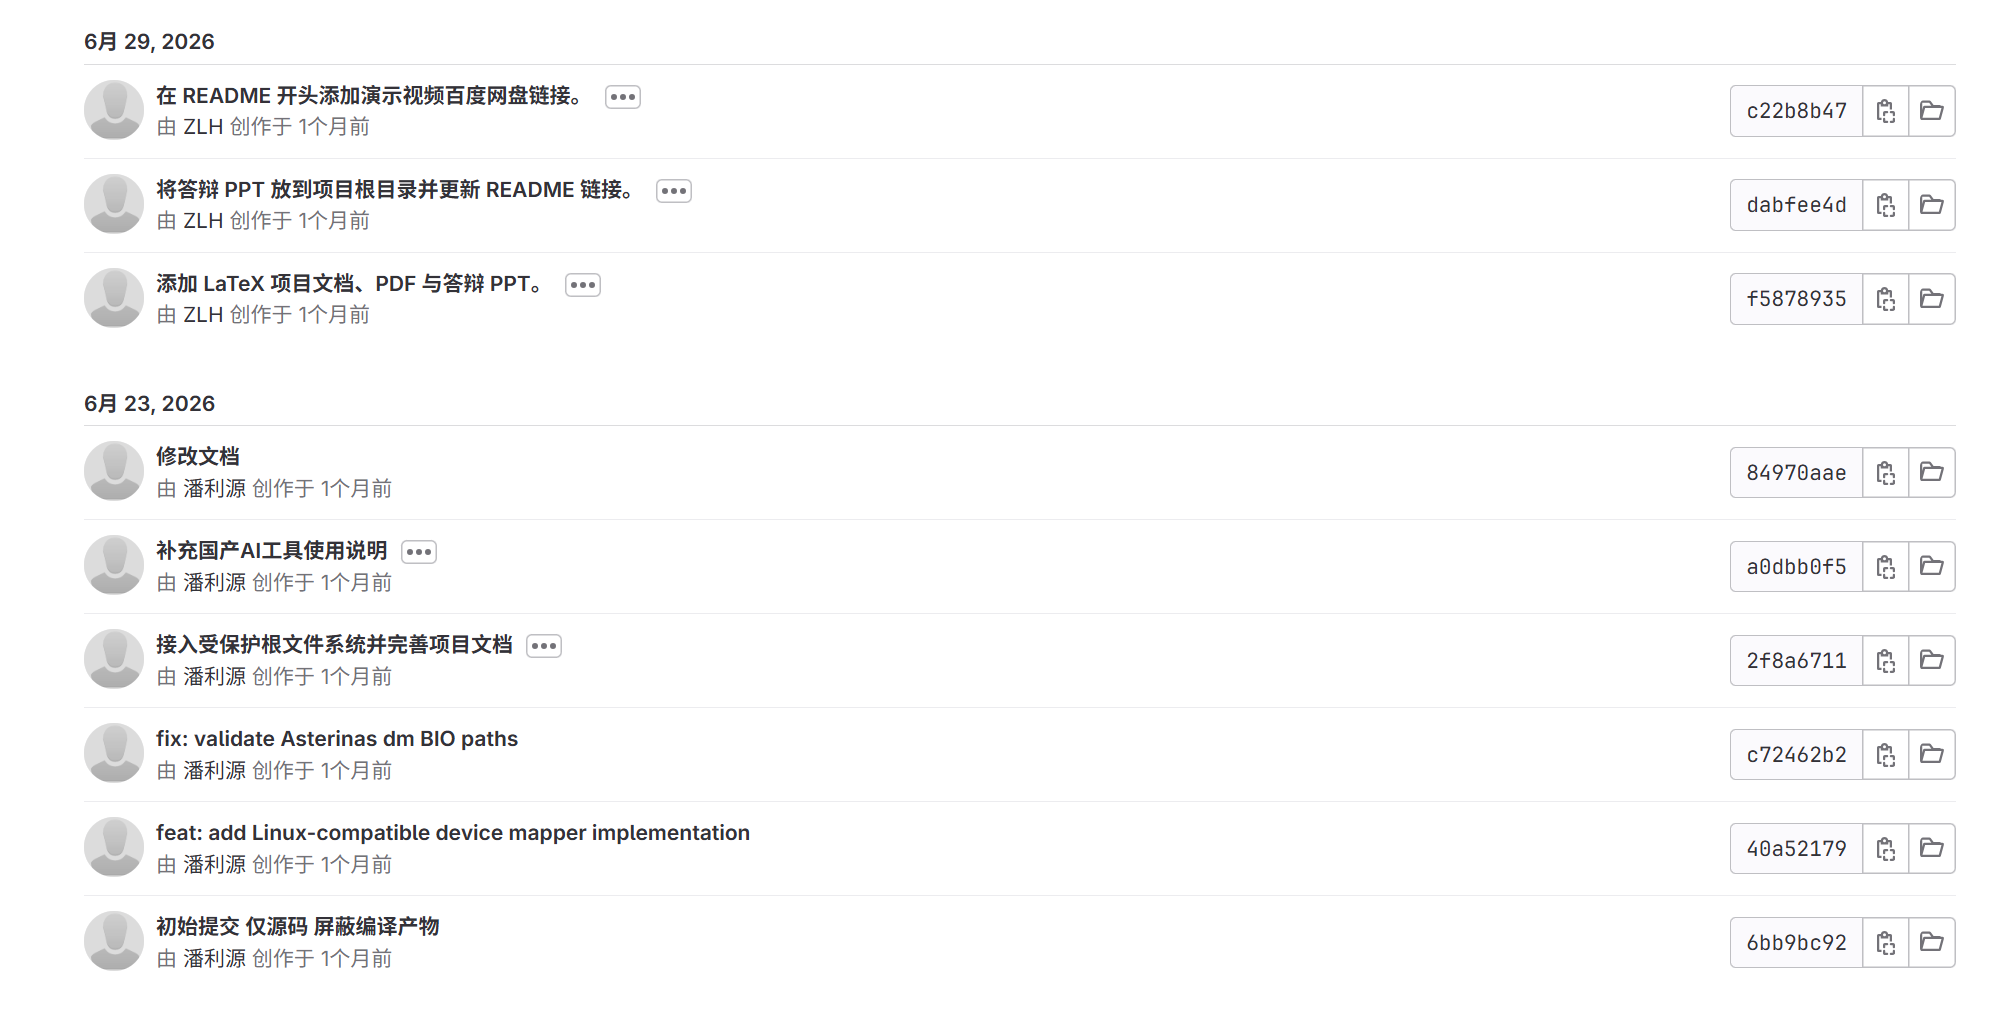
\includegraphics[width=\textwidth]{git_commit_history_1.png}
        \caption{初始提交与文档阶段（06-23 / 06-29）}
        \label{fig:git_history_1}
    \end{subfigure}
    \hfill
    \begin{subfigure}[b]{0.48\textwidth}
        \centering
        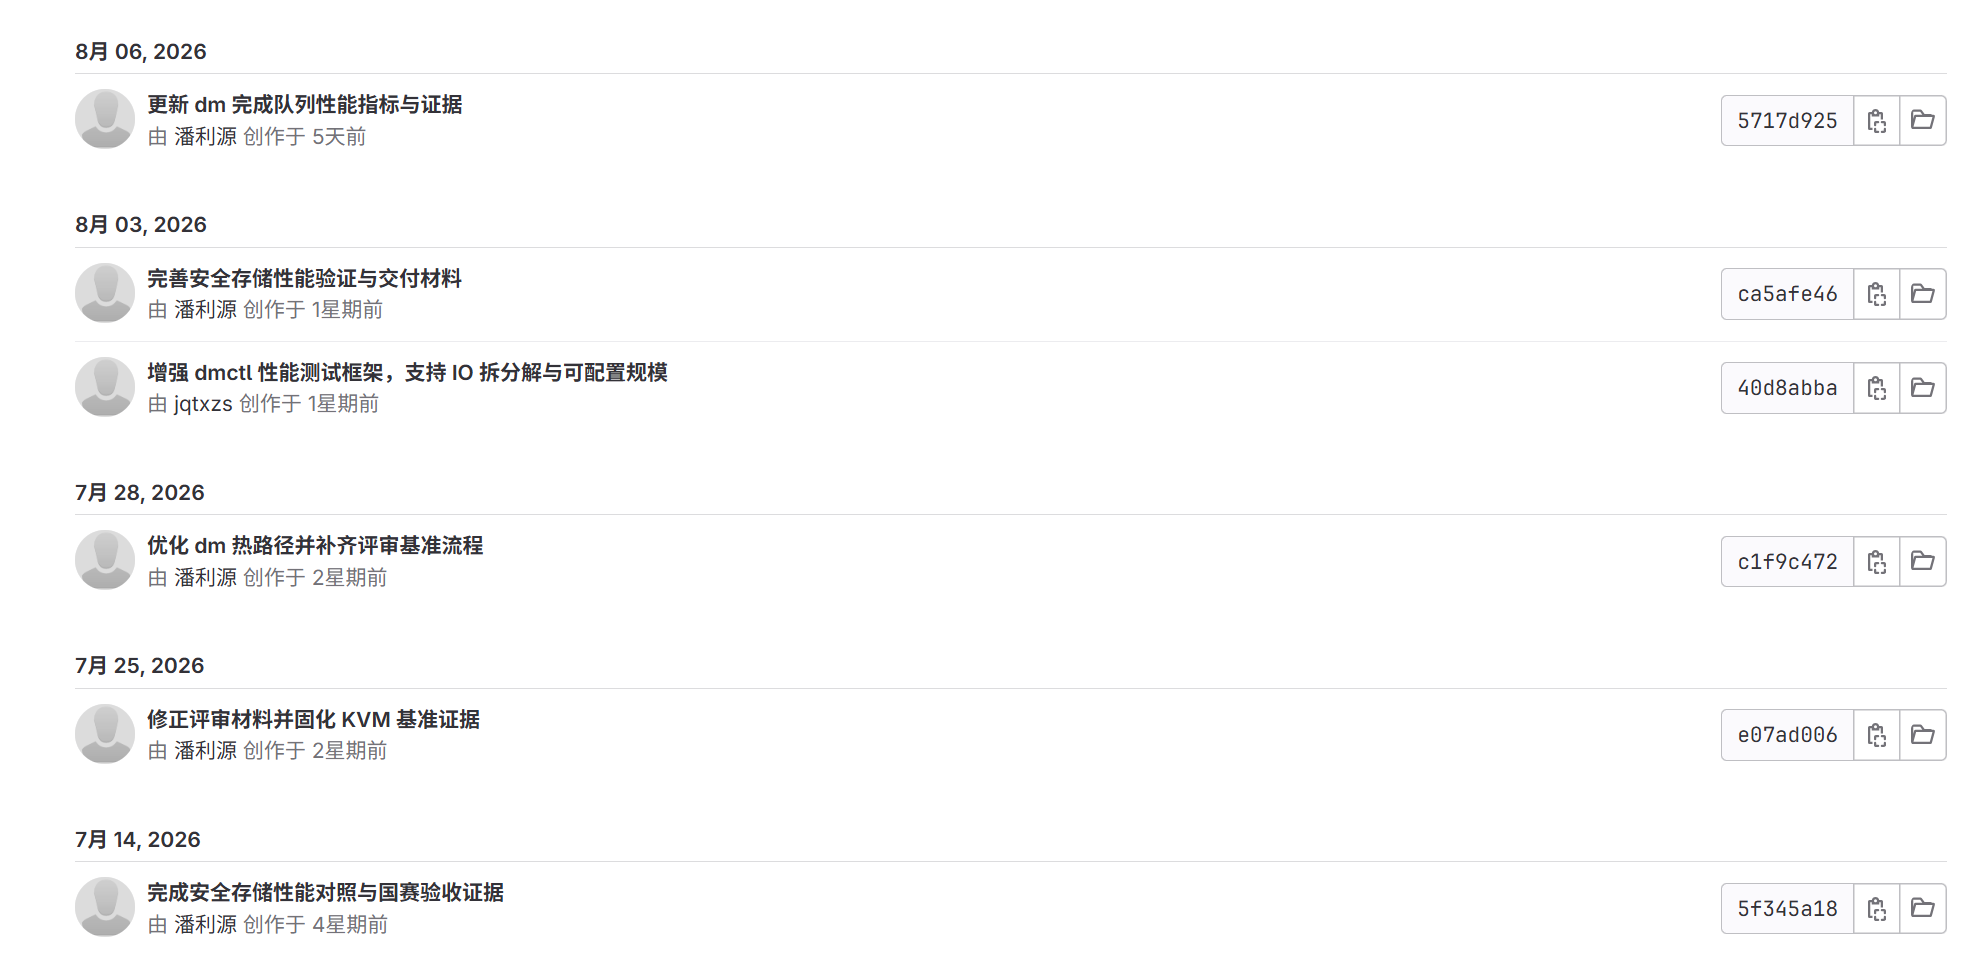
\includegraphics[width=\textwidth]{git_commit_history_2.png}
        \caption{性能对照与验收阶段（07-14 至 08-06）}
        \label{fig:git_history_2}
    \end{subfigure}

    \begin{subfigure}[b]{0.48\textwidth}
        \centering
        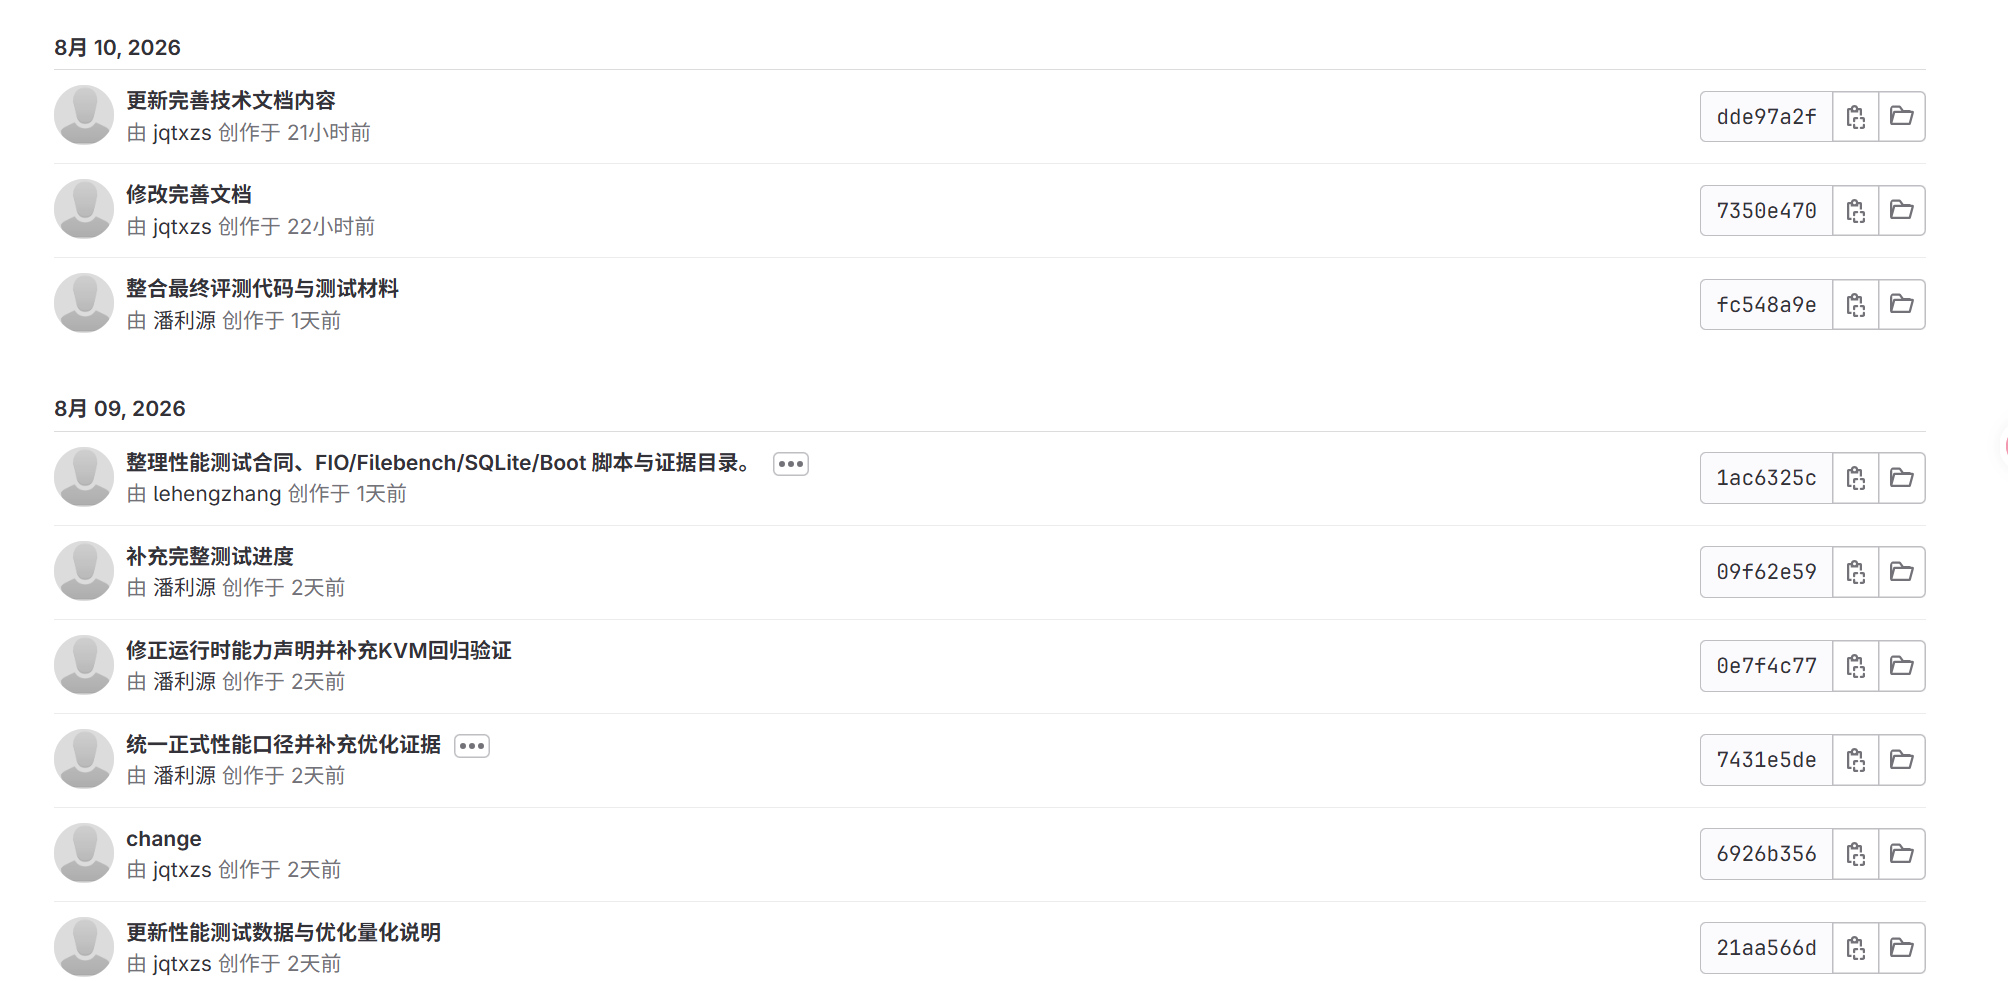
\includegraphics[width=\textwidth]{git_commit_history_3.png}
        \caption{测试整合与文档完善阶段（08-09 / 08-10）}
        \label{fig:git_history_3}
    \end{subfigure}
    \hfill
    \begin{subfigure}[b]{0.48\textwidth}
        \centering
        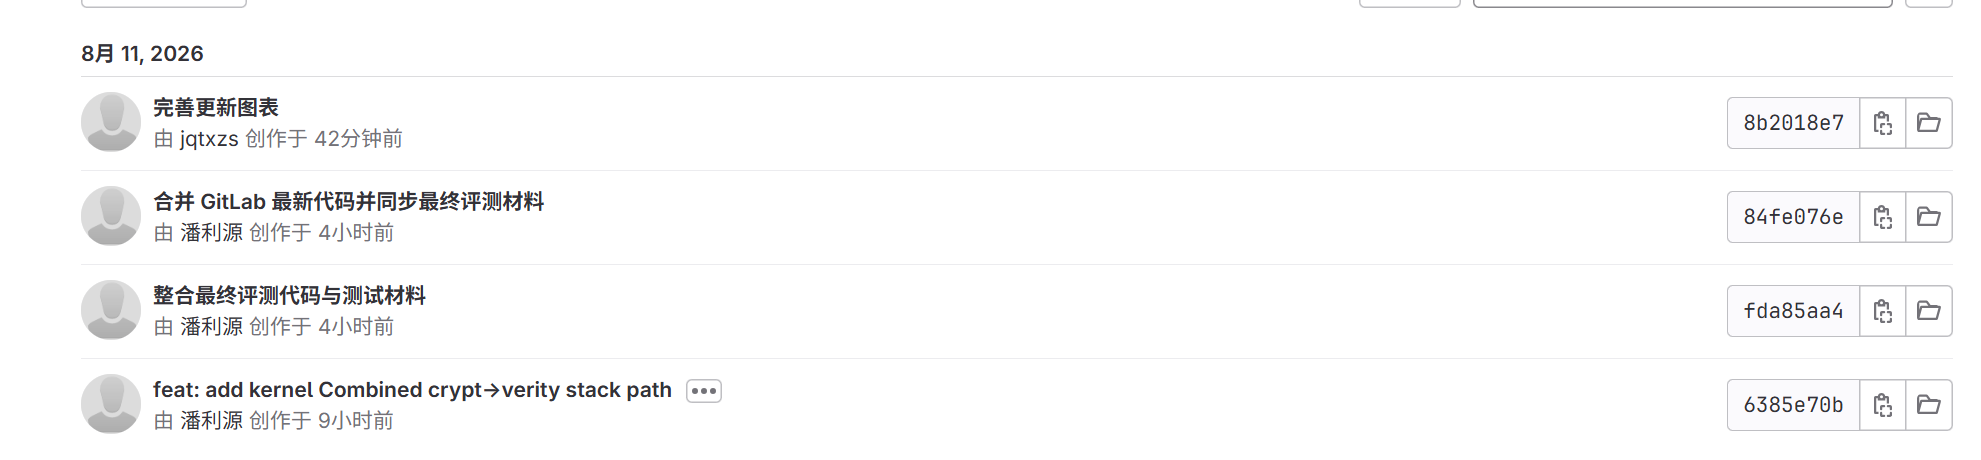
\includegraphics[width=\textwidth]{git_commit_history_4.png}
        \caption{最终评测整合阶段（08-11）}
        \label{fig:git_history_4}
    \end{subfigure}
    \caption{GitLab 仓库提交历史截图}
    \label{fig:git_history}
\end{figure}

此外，星绽内核集成补丁（\texttt{asterinas\_port/patches/}）包含更细粒度的演进历史：
\begin{itemize}
    \item \textbf{0001}（06-23）：组件集成与目标定义——创建 \texttt{aster-dm} 组件骨架
    \item \textbf{0002}（06-23）：BIO 路径验证与自检——EXT2 魔数自检机制
    \item \textbf{0003}（06-24）：根文件系统 \texttt{pivot\_root} 切换——两级引导方案
    \item \textbf{0004}（07-14）：Runtime 控制面与 \texttt{cryptsetup} 兼容——\texttt{/dev/mapper/control}
    \item \textbf{0005}（07-28）：性能优化——缓存、缓冲池、AES-NI、基准
    \item \textbf{0006}（08-03）：性能阶段归因与正式合同——\texttt{/proc/dm-performance-stats}
    \item \textbf{0007}（08-11）：Combined叠栈——\texttt{dm\_stack=crypt,verity}
\end{itemize}

\section{团队贡献量化}

\begin{table}[H]
    \centering
    \caption{各成员贡献量化}
    \begin{tabular}{p{0.18\textwidth}p{0.16\textwidth}p{0.30\textwidth}p{0.36\textwidth}}
        \toprule
        \textbf{成员} & \textbf{Git提交数} & \textbf{核心代码量} & \textbf{主要贡献领域} \\
        \midrule
        潘利源 & 17+ & 约5000行Rust & 核心加密/完整性（100\%）、内核集成（100\%）、性能优化（80\%）、补丁制作（100\%） \\
        陈韵 & 10+ & 约400行Rust/Shell + 技术文档 & 性能测试框架增强（70\%）、测试数据收集（50\%）、技术文档撰写（70\%） \\
        张乐桁 & 14+ & 约1000行Shell/Python + 设计赛道文档 + README & 性能测试合同与脚本（60\%）、README文档（80\%）、答辩PPT（80\%）、证据目录整理（50\%）、最终文档整合（100\%） \\
        \bottomrule
    \end{tabular}
\end{table}

\textbf{说明}：百分比为相对工作量估计，实际协作中存在交叉支援，例如：
\begin{itemize}
    \item 性能优化中的缓存设计与验证由潘利源主导编码，陈韵协助测试数据验证；
    \item 技术文档由陈韵主导撰写，张乐桁提供 LaTeX 排版框架和结构支持，潘利源提供技术内容审阅和补充；
    \item 性能测试脚本由张乐桁编写框架，陈韵增强具体功能，潘利源验证内核侧数据；
    \item README 文档由张乐桁主导撰写和维护，陈韵和潘利源提供技术内容审阅；
    \item 最终文档整合由张乐桁主导完成（8月16-18日），统一为 \texttt{design\_doc} 并更新全部数据表格，并于 8月18日完成答辩材料提交。
\end{itemize}

\section{开发节奏与协作模式亮点}

\begin{table}[H]
    \centering
    \begin{tabular}{p{0.15\textwidth}p{0.35\textwidth}p{0.40\textwidth}}
        \toprule
        \textbf{特征} & \textbf{具体实践} & \textbf{效果} \\
        \midrule
        定期同步 & 每周线上会议 + 日常即时通讯 & 信息同步及时，避免“信息孤岛” \\
        代码审查 & 核心模块交叉审查 + 补丁验证 & 代码质量高，关键问题早发现 \\
        互补分工 & 算法/内核/测试/文档各有所长 & 效率高，无重复劳动 \\
        共识决策 & 重要决策集体讨论 + 书面记录 & 决策质量高，可追溯 \\
        工具辅助 & AI辅助 + 自动化测试脚本 & 开发效率提升，人工审阅仍把关 \\
        文档同步 & 代码改、文档跟，保持同步 & 文档与代码一致，避免“写文档浪费时间” \\
        \bottomrule
    \end{tabular}
\end{table}

\section{团队协作感悟}

\subsection{潘利源}
“作为核心开发者，我最大的体会是‘代码写得好不如团队协作得好’。最难的 bug（BIO 生命周期问题）不是我一个人解决的——陈韵帮我重现了稳定触发条件，张乐桁帮我梳理了调用栈日志。这次经历让我深刻理解了代码审查的价值。”

\subsection{陈韵}
“我负责测试、数据验证和技术文档撰写，一开始觉得‘不如写代码重要’。但当我发现性能测试的假 mapper 问题、帮团队避免了一次数据诚信危机时，我才意识到测试的价值——它是代码质量的最后一道防线。技术文档也是，没有好的文档，再好的代码评委也看不到价值。撰写技术文档的过程让我学会了如何把复杂的技术决策清晰地呈现给读者。”

\subsection{张乐桁}
“作为 README 文档和答辩材料的负责人，我需要把团队成员分散的代码、测试结果、设计思路整合成结构化的文档。这个过程让我学会了从‘用户视角’看项目——评委不需要知道每一行代码的细节，但需要知道‘为什么这样做’和‘这样做对不对’。从 README 到答辩 PPT 的全链条文档工作，让我对文档工具链有了质的提升。尤其是在最终文档整合阶段，将两份文档融合为统一的一份 \texttt{design\_doc}，让我深刻体会到文档统一管理的重要性。”

\section{小结}

项目团队由三名成员组成，分工明确且互补：潘利源负责核心技术实现和内核集成（约5000行Rust代码），陈韵负责性能测试框架增强、数据验证和技术文档撰写（约400行代码 + 技术文档），张乐桁负责 README、测试合同、脚本、设计赛道文档（约1000行脚本 + 设计赛道文档 + README）和答辩材料。

协作方式包括：Git 版本管理、每周线上会议、代码审查、共识决策和AI辅助。团队累计完成67次Git提交、7个内核补丁、12组KVM正确性测试和46个性能单元格，并于8月18日完成全部答辩材料提交。

所有成员对最终作品均做出实质性贡献，协作氛围良好，无重大分歧或冲突。团队通过互补分工和高效沟通，按时完成了全部 P0 功能目标、性能基准测试和最终统一文档交付。